\subsection{Networked SBCs}

Figure \ref{fig:arch_03} illustrates the components of the networked SBD devices. A processing back application can hold any number of processors that each register thier services to the Zeroconf / Bonjour daemon installed on the devices operating system. The Zeroconf / Bonjour daemon broadcasts the availablilty, type and the port numbers of each of the processors available.

\begin{figure}[H]
    \centering
    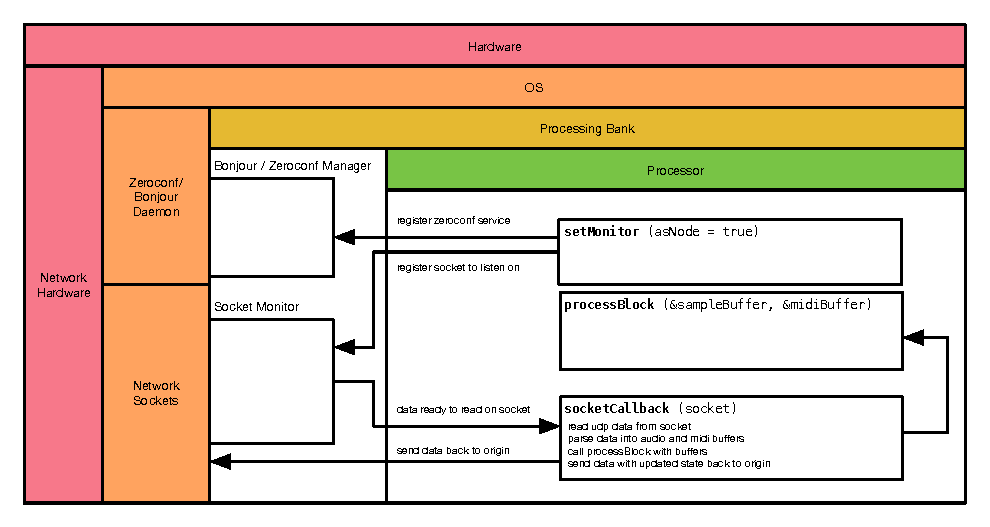
\includegraphics[width=\textwidth]{assets/architecture_03.pdf}
    \caption{SBC Processor Overview}
    \label{fig:arch_03}
\end{figure}



The processor also registers an open socket and itself as that socket's listener at the appliation's socket monitor module. The socket monitor holds an array of sockets and a reference to each listener. It performs a select() on the array of sockets and waits. When data arrives at any of the sockets, the select() is unblocked and the socket monitor notifies the corresponding listener via callback that data is available.

The corresponding processor is notified via the callback function, it reads the data, parses the audio and midi buffers, then perform a processBlock function on the buffers. The results and updatad state information is that passed back to the origin.

